% Santos. Include from a document with graphicx, booktabs, amsmath and float.
\subsection{Adiabatic electrons at zero temperature gradients}\label{sec:additional-adiabatic-zero}
We evolved one kinetic species, deuterium with input mass 2 and charge $+1$, with implicit Boltzmann electrons and $\tau=1$. The equilibrium electron density is the neutralizing background and shares the ion equilibrium density gradient. Only the ion gradient enters a kinetic species block. We used uniform species temperatures, the archived dipole geometry and dimensionless normalization, $(l_v,l_w)=(3.5,12.25)$, $k_y\rho_{\rm ref}=0.7$, $\beta=0$ and zero collisions.

The four $24/64/24$ cases at \texttt{hyp\_z=0} reached $\widehat t\simeq54.62$ with $\Delta\widehat t=0.04965703591$, before the nominal deuterium recurrence time $56.55$. GENE did not establish a mode at any of the four points. We projected the complex field onto the corresponding $\phi$ profile near $\widehat t=52$ and fit the log modulus and unwrapped phase. The slopes in the table use $44\le\widehat t\le52$. Ranges compare windows $30$--$40$, $36$--$44$ and $44$--$52$.

\begin{center}\small
\begin{tabular}{@{}rrrrrl@{}}
\toprule
$\omega_{n,D}$ & Fit $\widehat\gamma$ & Fit $\widehat\omega_r$ & $\widehat\gamma$ range & Wall (s) & Mode\\
\midrule
0.2 & -0.0640 & -0.0331 & $[-0.0673,\ -0.0539]$ & 40.3 & Unresolved\\
0.6 & +0.0271 & -0.0323 & $[-0.0159,\ +0.0271]$ & 39.8 & Unresolved\\
1 & +0.0215 & -0.1306 & $[-0.0196,\ +0.0237]$ & 48.1 & Unresolved\\
1.5 & -0.0259 & -0.3371 & $[-0.0259,\ +0.0133]$ & 29.4 & Unresolved\\
\bottomrule
\end{tabular}

\end{center}

\begin{figure}[H]\centering
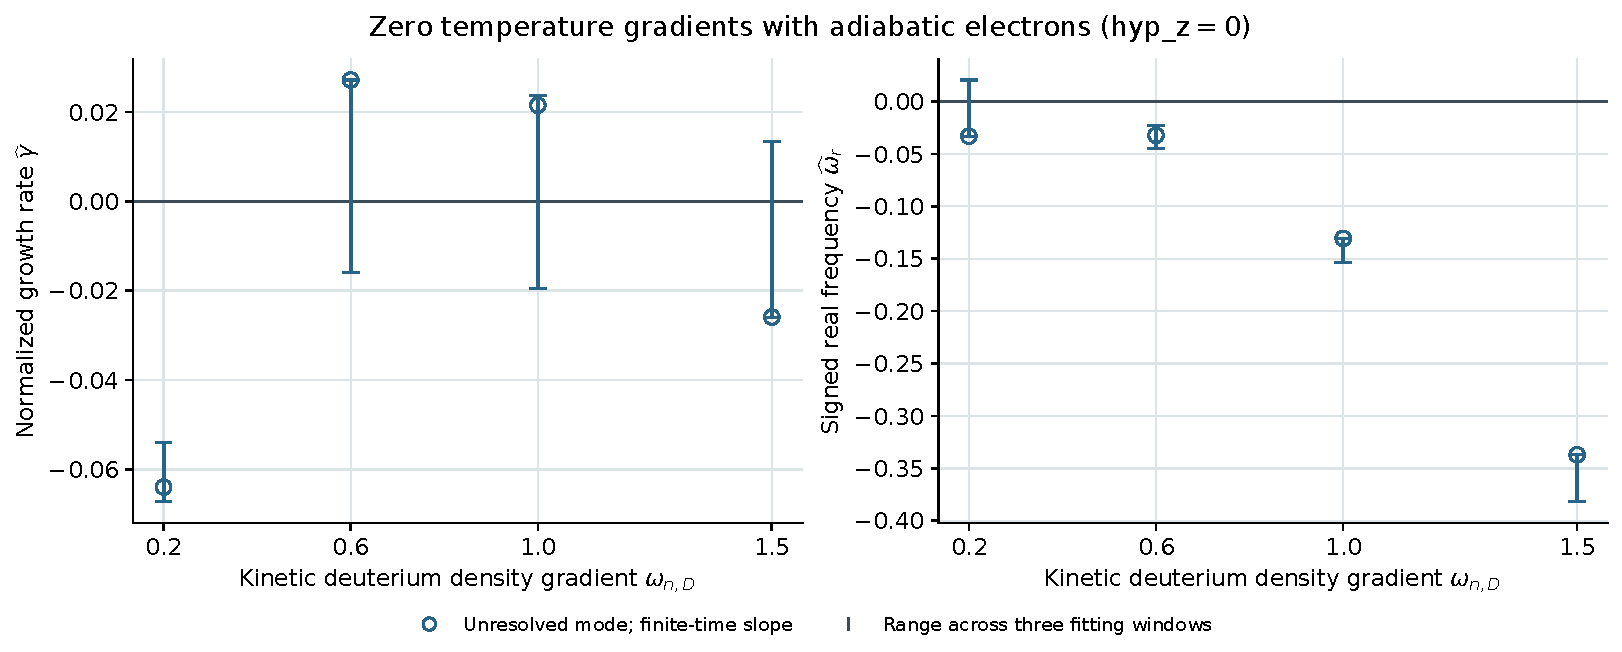
\includegraphics[width=\linewidth]{Figures/A_01_growth_and_signed_frequency.pdf}
\caption{GENE IV finite-time growth and signed phase slopes. Hollow markers indicate unresolved modes; bars show fitting-window ranges. Contributor: Santos.}
\label{fig:additional-adiabatic-slopes}
\end{figure}
